\section{What is a transfer function?}

A transfer function maps an input to an output in the Laplace domain. This is
essentially a two-dimensional frequency domain on the complex plane (real
numbers on the x-axis and imaginary numbers on the y-axis). These can be
obtained by applying the Laplace transform to a differential equation and
rearranging the terms to obtain a ratio of the output variable to the input
variable. Equation \ref{eq:transfer_func} is an example of a transfer function.

\begin{equation} \label{eq:transfer_func}
  H(s) = \frac{(s-9+9i)(s-9-9i)}{s(s+10)}
\end{equation}

Roots of the numerator and denominator are called residues. Residues on the top
are called zeroes while residues on the bottom are called poles. This is due to
poles making the expression approach infinity for values of $s$ that make the
residue zero (they look like poles of a circus tent on a 3D graph). Similar
logic applies to zeroes. Imaginary roots always come in complex conjugate pairs
(e.g., $-2 + 3i$, $-2 - 3i$).

\subsection{Transfer functions in feedback}

For \glspl{controller} to do their job, they must be placed in positive or
negative feedback with the \gls{plant} (positive or negative depends on the
\gls{plant} in question). The transfer function of figure
\ref{fig:feedback_loop}, a control system diagram with feedback, from input to
output is

\begin{equation}
  G_{cl}(s) = \frac{Y(s)}{X(s)} = \frac{P_1}{1 + P_1 P_2}
\end{equation}

The numerator is the \gls{open-loop gain} and the denominator is the gain around
the feedback loop, which may include parts of the \gls{open-loop gain} (see
appendix \ref{sec:app_tf_feedback_deriv} for a derivation). Plants are generally
denoted with the letter $G$. As another example, the transfer function from the
input to the error is

\begin{equation}
  G_{cl}(s) = \frac{E(s)}{X(s)} = \frac{1}{1 + P_1 P_2}
\end{equation}

The roots of the denominator of $G_{cl}(s)$ are different from those of the
open-loop transfer function $P_1(s)$. These are called the closed-loop poles.

\section{Locations of Poles and Zeroes}

The locations of the closed-loop poles in the complex plane determine the
stability of the \gls{system}. Each pole represents a frequency mode of the
\gls{system}, and their location determines how much of each response is induced
for a given input frequency.

\begin{figure}[H]
  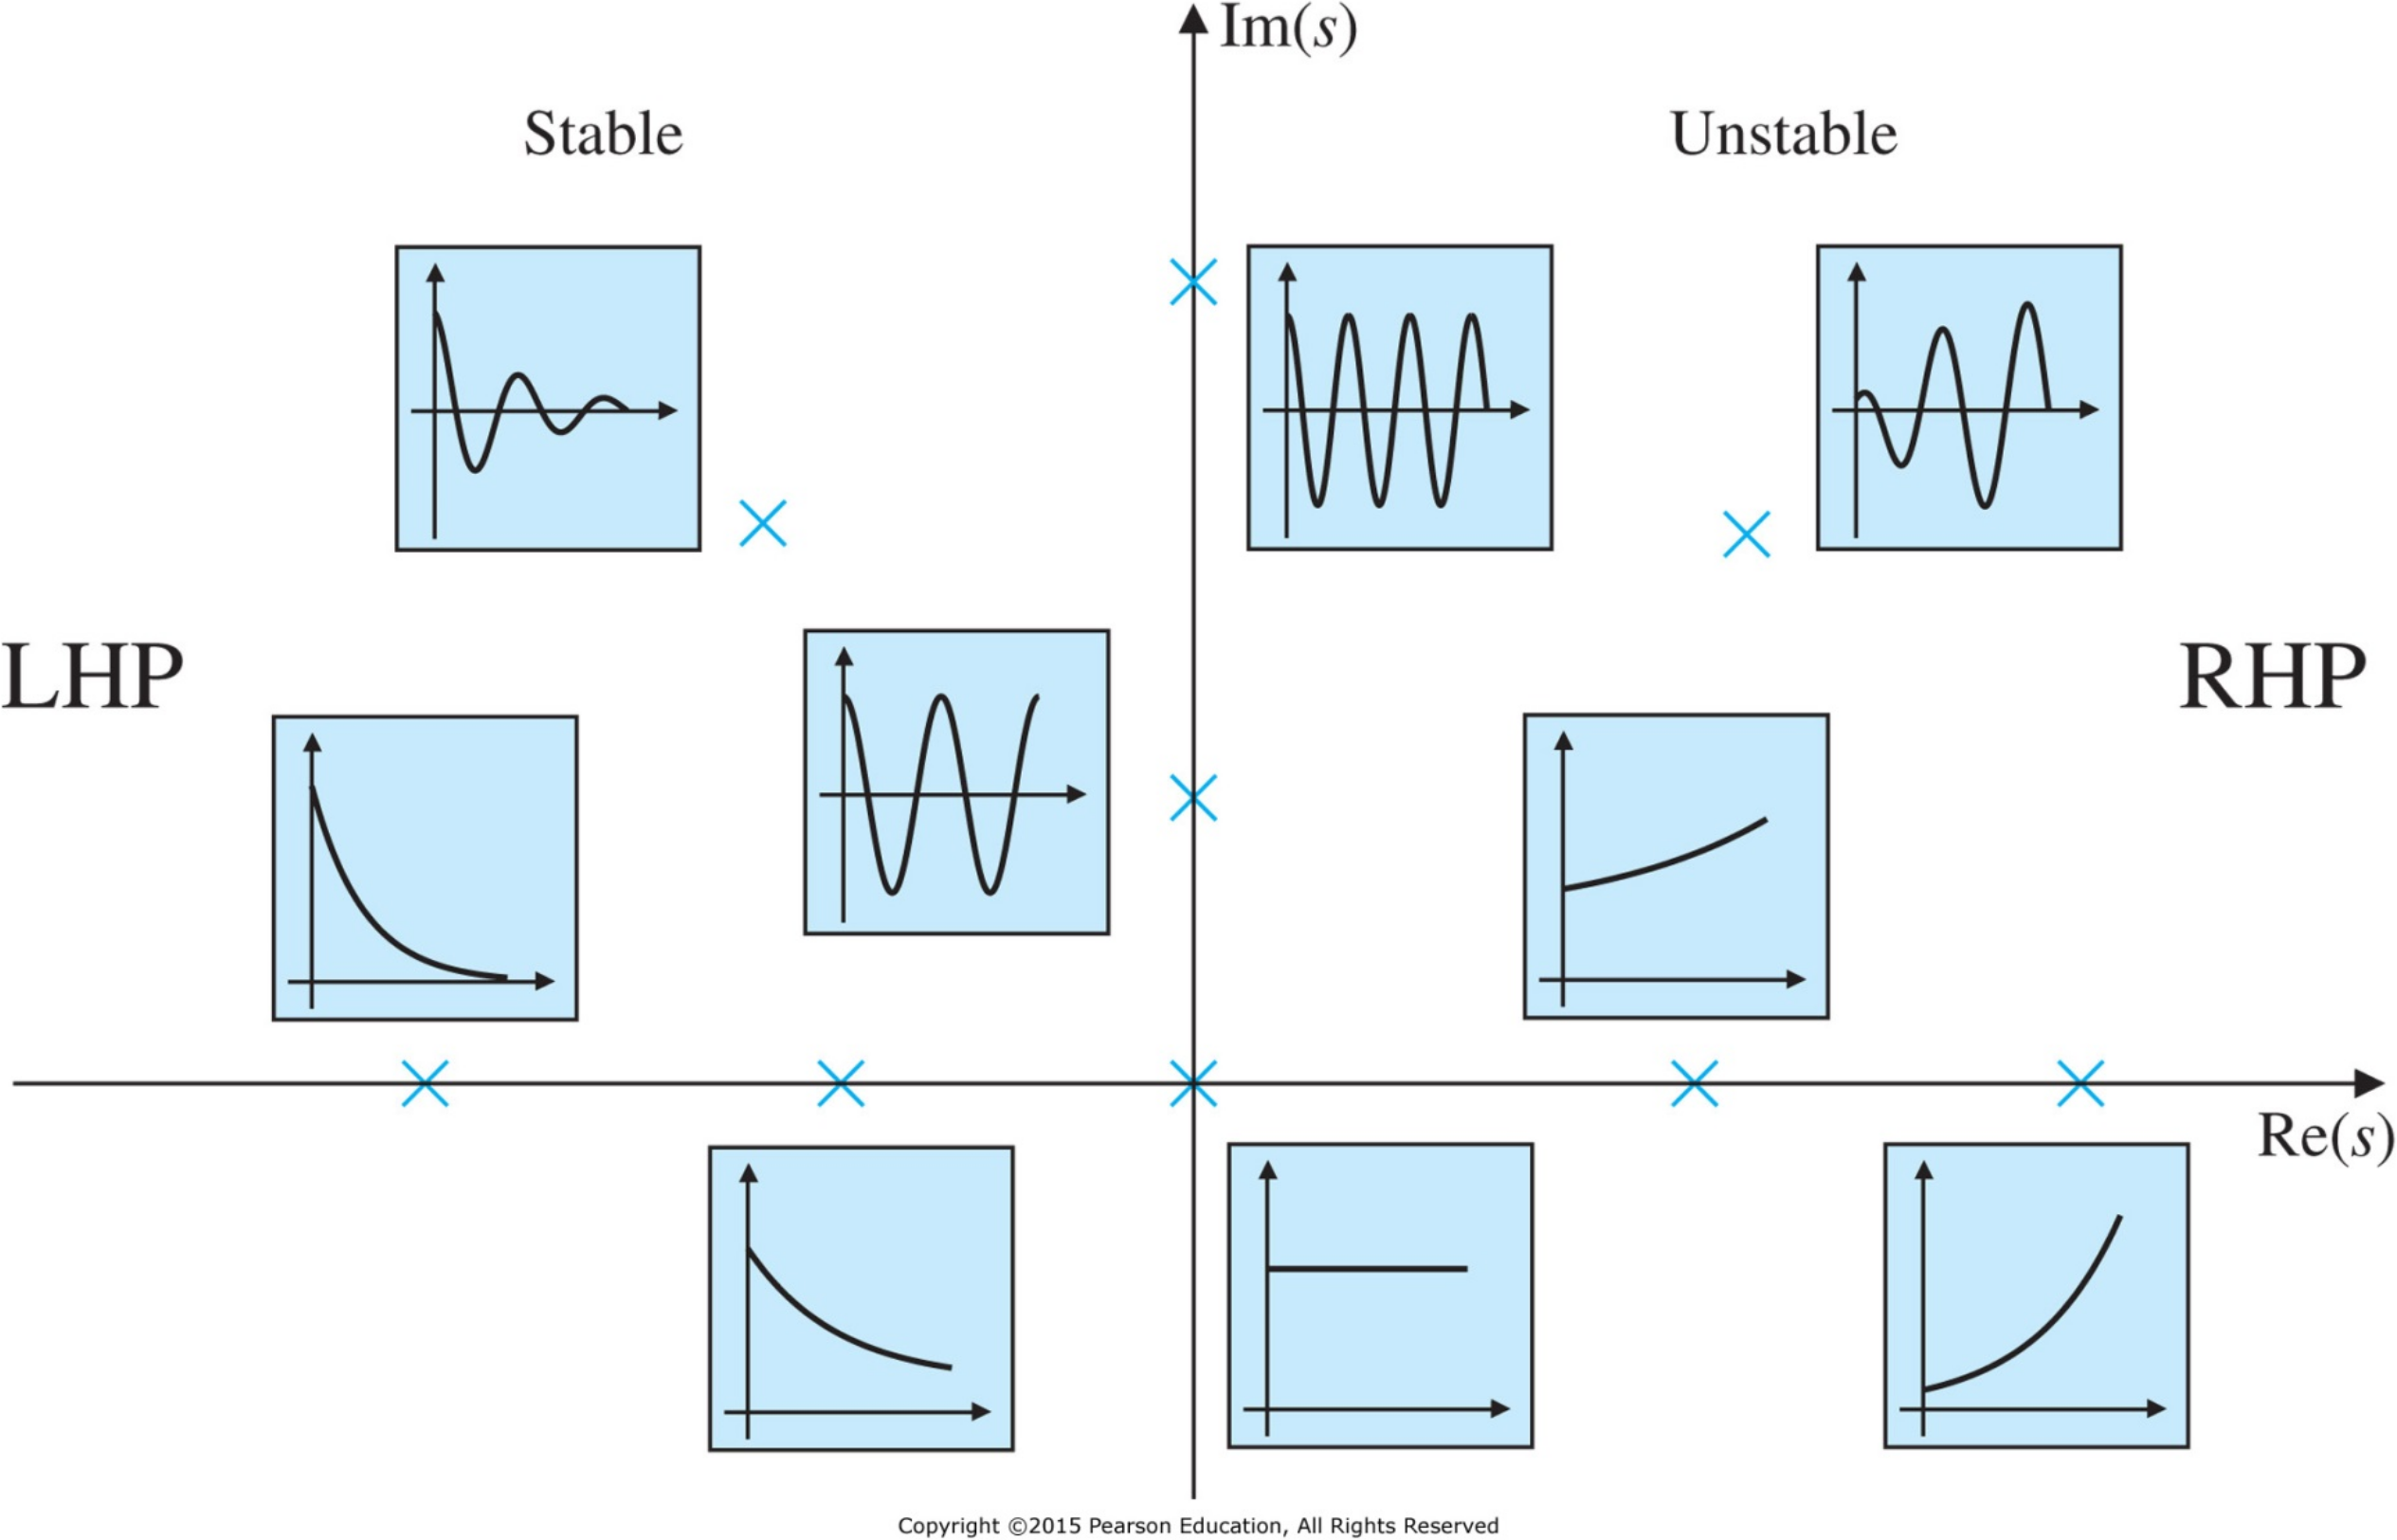
\includegraphics[width=\linewidth]{figs/ResponseVsPoleLocations.png}
  \caption{System responses vs pole locations \cite{bib:pole_locations}}
\end{figure}

\begin{table}[ht]
  \caption{Pole location and stabilty}
  \renewcommand{\arraystretch}{1.5}
  \centering
  \begin{tabular}{|ll|}
    \hline
    \rowcolor{lightblue}
    \textbf{Location} & \textbf{Stability} \\
    \hline
    Left-Half-plane (LHP) & Stable \\
    Imaginary axis & Marginally stable \\
    Right Half-plane (RHP) & Unstable \\
    \hline
  \end{tabular}
  \label{tab:pole_locations}
\end{table}

When a system is stable, its output may oscillate but it converges to
steady-state. When a system is marginally stable, its output oscillates at a
constant amplitude forever. When a system is unstable, its output grows without
bound.

\subsection{Root locus}

In closed-loop, the poles and zeroes can be moved around by the chosen
controller. The root locus shows where they will go as the controller gain is
increased. Figure \ref{fig:poster_rlocus} shows the root locus of the transfer
function from equation (\ref{eq:transfer_func}).

\begin{figure}[H]
  \def\svgwidth{\linewidth}
  \import{}{root_locus.pdf_tex}
  \caption{Root locus of equation (\ref{eq:transfer_func}). See snippet
    \ref{snip:poster_rlocus}.}
  \label{fig:poster_rlocus}
\end{figure}

\begin{snippet}
  \caption{Root locus in Python}
  \label{snip:poster_rlocus}
  \includecode[Python]{code/root_locus.py}
\end{snippet}

As the controller gain increases, the poles move toward the zeroes. In this
case, the \gls{system} eventually becomes unstable. \\

\textbf{Note:} If poles are much farther left in the LHP than the typical
\gls{system} dynamics exhibit, they can be considered negligible. Every
\gls{system} has some form of unmodeled high frequency, non-linear dynamics, but
they can be safely ignored depending on the operating regime.

\subsubsection{Non-minimum phase zeroes}

While poles in the RHP are unstable, the same is not true for zeroes. They can
be characterized by the \gls{system} initially moving in the wrong direction
before heading toward the \gls{reference}. Since the poles always move toward
the zeroes, zeroes impose a "speed limit" on the \gls{system} response because
it takes a finite amount of time to move the wrong direction, then change
directions. \\

One example is bicycle steering. Try riding a bicycle without holding the handle
bars, then poke the right handle; the bicycle turns right.

\section{Steady-state error}

To demonstrate the problem of \gls{steady-state error}, we will use a DC brushed
motor controlled by a velocity PID controller. A DC brushed motor has a transfer
function from voltage ($V$) to angular velocity ($\dot{\theta}$) of

\begin{equation}
  G(s) = \frac{\dot{\Theta}(s)}{V(s)} = \frac{K}{(Js+b)(Ls+R)+K^2}
\end{equation}

First, we'll try controlling it with a P controller defined as

\begin{equation*}
  K(s) = K_p
\end{equation*}

When these are in unity feedback, the transfer function from the input voltage
to the error is

\begin{align*}
  \frac{E(s)}{V(s)} &= \frac{1}{1 + K(s)G(s)} \\
  E(s) &= \frac{1}{1 + K(s)G(s)} V(s) \\
  E(s) &= \frac{1}{1 + (K_p) \left(\frac{K}{(Js+b)(Ls+R)+K^2}\right)} V(s) \\
  E(s) &= \frac{1}{1 + \frac{K_p K}{(Js+b)(Ls+R)+K^2}} V(s)
\end{align*}

The steady-state of a transfer function can be found via

\begin{equation}
  \lim_{s\to0} sH(s)
\end{equation}

\begin{align}
  e_{ss} &= \lim_{s\to0} sE(s) \nonumber \\
  e_{ss} &= \lim_{s\to0} s \frac{1}{1 + \frac{K_p K}{(Js+b)(Ls+R)+K^2}} V(s)
    \nonumber \\
  e_{ss} &= \lim_{s\to0} s \frac{1}{1 + \frac{K_p K}{(Js+b)(Ls+R)+K^2}}
    \frac{1}{s} \nonumber \\
  e_{ss} &= \lim_{s\to0} \frac{1}{1 + \frac{K_p K}{(Js+b)(Ls+R)+K^2}}
    \nonumber \\
  e_{ss} &= \frac{1}{1 + \frac{K_p K}{(J(0)+b)(L(0)+R)+K^2}} \nonumber \\
  e_{ss} &= \frac{1}{1 + \frac{K_p K}{bR+K^2}} \label{eq:ss_nonzero}
\end{align}

Notice that the \gls{steady-state error} is non-zero. To fix this, an integrator
must be included in the controller.

\begin{equation*}
  K(s) = K_p + \frac{K_i}{s}
\end{equation*}

The same steady-state calculations are performed as before with the new
controller.

\begin{align*}
  \frac{E(s)}{V(s)} &= \frac{1}{1 + K(s)G(s)} \\
  E(s) &= \frac{1}{1 + K(s)G(s)} V(s) \\
  E(s) &= \frac{1}{1 + \left(K_p + \frac{K_i}{s}\right)
    \left(\frac{K}{(Js+b)(Ls+R)+K^2}\right)} \left(\frac{1}{s}\right) \\
  e_{ss} &= \lim_{s\to0} s \frac{1}{1 + \left(K_p + \frac{K_i}{s}\right)
    \left(\frac{K}{(Js+b)(Ls+R)+K^2}\right)} \left(\frac{1}{s}\right) \\
  e_{ss} &= \lim_{s\to0} \frac{1}{1 + \left(K_p + \frac{K_i}{s}\right)
    \left(\frac{K}{(Js+b)(Ls+R)+K^2}\right)} \\
  e_{ss} &= \lim_{s\to0} \frac{1}{1 + \left(K_p + \frac{K_i}{s}\right)
    \left(\frac{K}{(Js+b)(Ls+R)+K^2}\right)} \frac{s}{s} \\
  e_{ss} &= \lim_{s\to0} \frac{s}{s + \left(K_p s + K_i\right)
    \left(\frac{K}{(Js+b)(Ls+R)+K^2}\right)} \\
  e_{ss} &= \frac{0}{0 + (K_p (0) + K_i)
    \left(\frac{K}{(J(0)+b)(L(0)+R)+K^2}\right)} \\
  e_{ss} &= \frac{0}{K_i \frac{K}{bR+K^2}} \\
\end{align*}

The denominator is non-zero, so $e_{ss} = 0$. Therefore, an integrator is
required to eliminate \gls{steady-state error} in all cases for this model. \\

It should be noted that $e_{ss}$ in equation (\ref{eq:ss_nonzero}) approaches
zero for $K_p = \infty$. This is known as a bang-bang controller. In practice,
an infinite switching frequency cannot be achieved, but it may be close enough
for some performance specifications.

\section{Going Digital}

The complex plane discussed so far deals with continuous \glspl{system}. In
decades past, \glspl{plant} and controllers were implemented using analog
electronics, which are continuous in nature. Nowadays, microprocessors can be
used to achieve cheaper, less complex controller designs. However, this comes
with drawbacks. \\

Since a microcontroller performs discrete steps, there is phase loss introduced
in the controller. Large amounts of phase loss can make a stable controller in
the continuous domain go unstable in discrete. Here are a few ways to combat
this.

\begin{itemize}
  \item Run the controller with a high sample rate.
  \item Designing the controller in the analog domain with enough phase margin
    to compensate for any phase loss that occurs as part of discretization.
  \item Convert the \gls{plant} to the digital domain and design the controller
    completely in the digital domain.
\end{itemize}

\subsection{s-plane to z-plane}

Transfer functions are converted to impulse responses using the Z-transform. The
s-plane's LHP maps to the inside of a unit circle in the z-plane. Here are a few
common points.

\begin{table}[ht]
  \caption{Mapping from s-plane to z-plane}
  \renewcommand{\arraystretch}{1.3}
  \centering
  \begin{tabular}{|cc|}
    \hline
    \rowcolor{lightblue}
    \textbf{s-plane} & \textbf{z-plane} \\
    \hline
    $(0, 0)$ & $(0, 1)$ \\
    imaginary axis & edge of unit circle \\
    $(0, -\infty)$ & $(0, 0)$ \\
    \hline
  \end{tabular}
  \label{tab:s-plane2z-plane}
\end{table}

You may notice that poles can be placed at $(0, 0)$ in the z-plane. This is
known as a deadbeat controller. An $\rm N^{th}$ order deadbeat controller decays
to the \gls{reference} in N timesteps. While this sounds great, there are other
considerations like actuation effort and robustness. These will be discussed in
detail with LQR controllers.
